%!TEX root = ../template.tex
%%%%%%%%%%%%%%%%%%%%%%%%%%%%%%%%%%%%%%%%%%%%%%%%%%%%%%%%%%%%%%%%%%%%
%% chapter2.tex
%% NOVA thesis document file
%%
%% Chapter with the template manual
%%%%%%%%%%%%%%%%%%%%%%%%%%%%%%%%%%%%%%%%%%%%%%%%%%%%%%%%%%%%%%%%%%%%

\typeout{NT FILE chapter2.tex}%

\chapter{Background}
\label{cha:background}

The present research work aims to propose an approach to improve requirements modeling by leveraging Generative AI (GAI) techniques to automate the generation of UML diagrams during the software design phase. The purpose of this chapter is to briefly introduce the main concepts in the field of software modeling that serve as the foundation for this thesis, namely tools, techniques, and approaches for translating requirements into design models, with a particular focus on UML class diagrams and their key components (classes, attributes, operations, and relationships). Additionally, we provide an overview of Generative AI and Retrieval-Augmented Generation (RAG), which form the core technologies employed in this research. This chapter also discusses related work and systematic methodologies, such as systematic mapping study, conducted to identify gaps and opportunities addressed in this thesis.

\iffalse
\section{Requirement Engineering}
\label{sec:requirement_engineering}

Requirements Engineering is the process that "covers all of the activities involved in discovering, documenting, and maintaining a set of requirements for a computer-based system" \cite{1BKotonya1998}. Its fundamental for identifying, eliciting, analysing, specifying, validating, what is needed from a system, identifying the system's constraints, and understand the motivation behind its development \cite{2BZave1997}. Requirements engineering assures that the features and functionalities asked by stakeholder are managed correctly, so the development team can accurately design and implement the system that meets stakeholders' and users' expectations \cite{3BNuseibeh2000}. 

\subsection{activities of requirement engineering}
The process is divided into 5 major activit \cite{4BSharma2013}:
\begin{enumerate}
    \item \textbf{Requirements elicitation:}Is the process that focuses on gathering information to gain knowledge about the project domain and requirements. It helps to better understand the needs and expectations of the stakeholders.
    \item \textbf{Analysis and Negotiation:}This second phase consists on solving the problems within the system requirements. During this phase if a requirement is considered incomplete, ambiguous and/or conflicting during the analysis, its referred back to elicitation. Negotiation part consists on finding an agreement with stakeholders to all be satisfied with the changes.
    \item \textbf{Documentation:} After the requirements are analyzed, it is fundamental to record them to make them formal, this way the team organizes the requirements in a way it ascertains their clarity, consistency and traceability, etc.
    \item \textbf{Requirement Validation:} This phase check that all the requirements identified in the previous process are complete, consistent and accurate. Also makes sure that are in accordance with the stakeholders needs and expectations.
    \item \textbf{Requirements Management:} Is the process of managing requirements throughout the software development process of managing the requirements throughout the software development process.
\end{enumerate}
These 5 phases constitute the general set of main activities in the requirements engineering process. They can be adapted to meet certain organization needs or changed depending on the system being developed. \cite{1BKotonya1998}
In this thesis, we will be focusing on the Documentation, we aim to help make the subprocess more efficient and more automated by automating the creation of the formal design models such as UML class diagrams. 
\fi
\section{Software Modeling}
\label{sec:software_modeling}

Modelling is a fundamental practice in science and engineering, used to create abstract representations of a system at varying levels of precision and detail. These models serve as analytical tools, enabling a deeper understanding of the system’s structure, behaviour, and constraints throughout its development process  \cite{5BGomaa2011}
This thesis will use Unified Modelling Language (UML) to produce design models from requirements.

Unified modelling language was developed to provide a standardized graphical language and notation for describing object-oriented models. UML notation is one of the most use language for describing software requirements, analysis and design models. 
The first time UML was introduced was by Grady Booch, James Rumbaugh, and Ivar Jacobson  in 1999 \cite{6BBooch1999} and after was officially adopted in January 1997 by OMG. In the OMG’S view, “modeling is the designing of software applications before coding.”.

Unified Modeling Language (UML) is not only used for object-oriented design but also for modeling and functional aspects of systems \cite{7BSergievskiy2018}. The current standard version, UML 2.5.1, continues to evolve and supports various diagrams for application development, including use case diagrams, class diagrams, object diagrams, communication diagrams, sequence diagrams, state machine diagrams, activity diagrams, composite structure diagrams, and deployment diagrams.In this thesis, we focus on class diagrams for  design modeling. Class diagrams are the most widely used UML diagrams \cite{8BImportanceClassDiagrams}, providing a visual representation of a system's structure by illustrating classes, their attributes, methods, and the relationships among them. In addition to aiding system visualization, class diagrams also serve as a documentation tool and design blueprint, ensuring consistency and alignment with the system's intended functionality.

\subsection{Benefits for developers and stakeholders}
Class diagrams present benefits for the developers and the stakeholders both benefit from clear communication, as it acts as a universal language, reducing the gap between technical and non-technical stakeholders. By providing a clear and concise visual representation, it guarantees that everyone involved is in understanding. Also, it helps identifying potential design issues early in the development process because of the clear and concise visualization of the design.
Additionally, class diagrams help assuring quality by for example ensuring that the system respects certain design principles or patterns, which can further improve the quality and maintenance of the software \cite{9BZapataBarra2018}.

\subsection{Core components of UML class diagrams}
In UML Class diagram, classes are represented as rectangular boxes, with their attributes and operations detailed inside. The relationships between class are represented using different types of connectors, which demonstrate structural and behavioural associations within the system. There are four primary types of relationships: associations, whole/part relationships, and generalization/specialization relationships and dependencies.
An association represents a static structural relationship between two or more classes. It defines how instances of one class are related to instances of another class \cite{5BGomaa2011}. Associations can have multiplicity, which specifies how many instance of one class can be associated with instance of another class, (see Figure~\ref{fig:UmlNotionRelationships}  a). The multiplicity of an association ca be optional (0..1), exactly one (1), zero or more (*), numerically specified (m..n), or one or more (1..*)
Whole/part relationships define hierarchical relationships between objects. There are, two types, Aggregation and Composition. Aggregation represents a weak relationship between the whole and its parts, where the part can exist independently of the whole. It is portraited with a hallow diamond at the end of the association. In contrast, composition represents a strong relationship where the part cannot exist independently of the whole. It is presented as a filled diamond at the end of the association (see Figure~\ref{fig:UmlNotionRelationships}  b).
Generalization/Specialization Hierarchy is an inheritance relationship, where a subclass inherits properties from a superclass. This allows for the reuse of common attributes and behaviors.It Is represented by an arrow joining the subclass (child) to the superclass (parent) (see Figure~\ref{fig:UmlNotionRelationships} c)
A dependency relationship, is often used to show how packages are related, and represents a weaker relationship where one class depends on another for its operation

\begin{figure}[htbp]
    \centering
    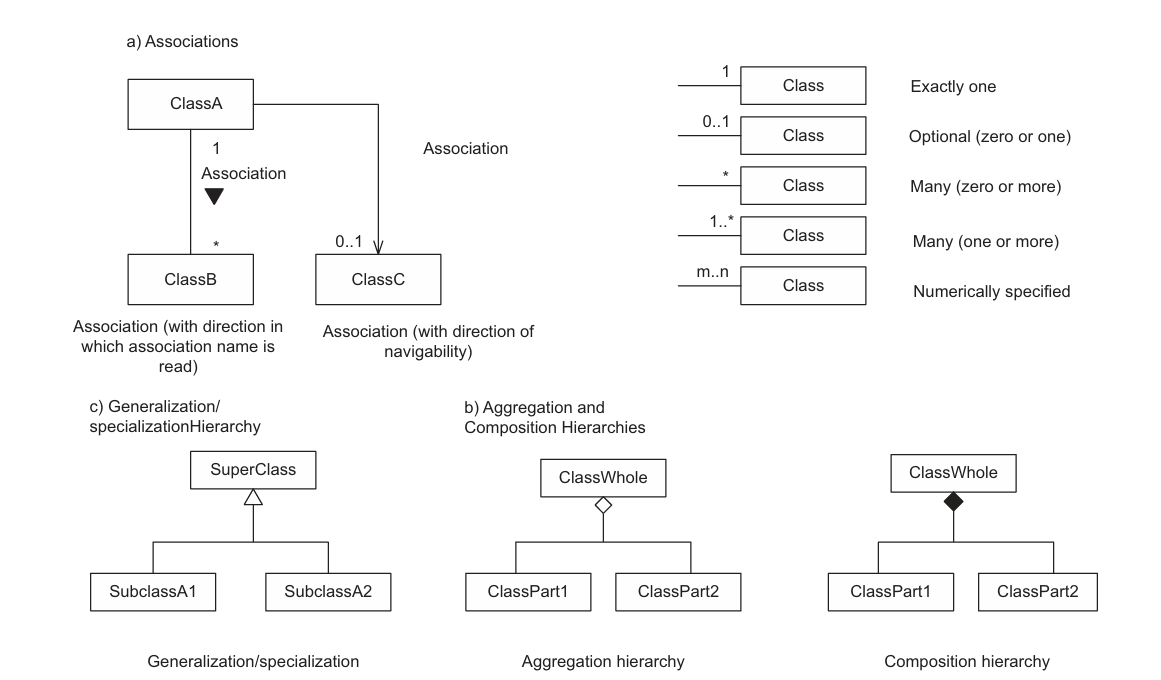
\includegraphics[width=0.8\linewidth]{Chapters/Figures/UMLnotation2.png} % Adjust width or use height
    \caption{ UML notation for relationships on a class diagram \cite{5BGomaa2011} }
    \label{fig:UmlNotionRelationships}
\end{figure}
\begin{figure}[htbp]
    \centering
    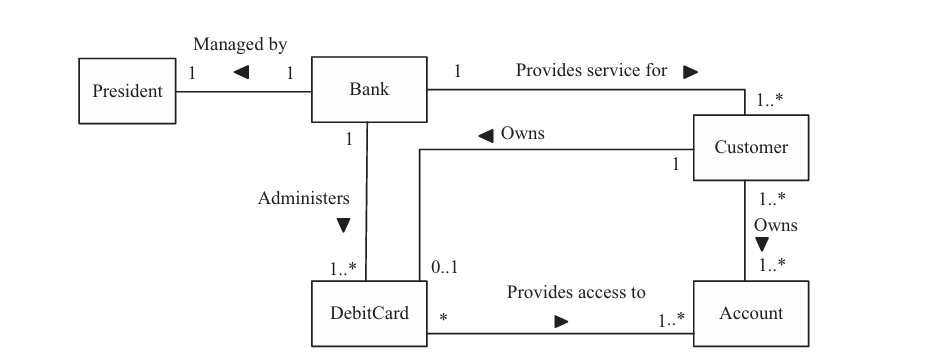
\includegraphics[width=0.8\linewidth]{Chapters/Figures/UMLnotation3.png} % Adjust width or use height
    \caption{ Example of relationships on a class diagram \cite{5BGomaa2011} }
    \label{fig:relationshipClassDiagram}
\end{figure}

\subsection{UML design class diagrams}
The design process involves several key steps to ensure that the diagram accurately models the system's domain and behavior. By following a structured approach, designers can systematically identify the key components, define their relationships, and establish clear interactions within the system. The following steps outline a methodical process for designing a UML class diagram:
\begin{enumerate}
    \item \textbf{Requirements Analysis:} understand the system's requirements by identifying the main entities or classes that will be part of the system.
    \item \textbf{Identifying Relationships:} identify how the class will interact with the others by determining the type of relationships.
    \item \textbf{Define Multiplicity:} determine the multiplicity of the association, i.e. specify how many instances of one class may relate to a single instance of another class \cite{5BGomaa2011}.
    \item \textbf{Add attributes and methods:} for each class list attribute (properties, fields) and methods (functions), it will have.
    \item \textbf{Draw the diagram:} begin by creating class boxes with their names. Next, add attributes and methods to define each class's structure and behavior. Finally, establish relationships between classes, ensuring proper associations, generalizations, and dependencies, while specifying multiplicity where necessary.
    \item \textbf{Review and refine:} review the diagram for accuracy, completeness, and consistency. Refine it as needed to ensure clarity and correctness.
 \end{enumerate}

There exists many different tools and software used to representing class diagrams, the most popular are Microsoft Visio \cite{microsoft_visio}, StarUML \cite{staruml}, PlantUML \cite{plantuml}, and Lucidchart \cite{lucidchart}.


\section{Large Language models (LLMs)}
\label{sec:large_language_models_llms}

LLMs are models trained on vast amounts of textual data that excel in NLP tasks \cite{10BScao2022}. They started to gain popularity after the release of OpenAI's ChatGPT model in November 2022, which is built using the transformer architecture. It exhibits capabilities such as creative writing, translation, instruction following, summarizing. 

While the LLMs can be powerful tools, they are only as good as the data they are trained on. If the training data is bias the outputs will be biases \cite{11BClusmann2023}. Therefore, overreliance on LLMs can lead to skill degradation and incorrect assessment \cite{12BLiyanage2023}. It is important to consider and assess the risk of using LLMs for specific use cases and check their outputs for errors.
\subsection{Architecture of LLMs}
The general architecture consists of multiple layers, including feedforward layers, embedding layers, and attention layers. The Transformer architecture, introduced by Vaswani et al. in 2017 \cite{13BVaswani2017}, revolutionized NLP by enabling efficient parallel processing of tokens. This capability is achieved its through its multi-head self-attention mechanism, which allows for parallelized model training on large datasets. Their architecture is composed of the following key components:
\begin{enumerate}
    \item \textbf{Input Embeddings}: This layer divides the input text into tokens that are embedded into a continuous vector representation that works as a lookup table.
    \item \textbf{Positional Encoding}: Encoding does not naturally encode the word order; therefore, positional information is added to each word’s vector representation so that it keeps the order of the words as in the text input.
    \item \textbf{Encoder}: Analyzes the input text and creates several hidden states that preserve the context and meaning of the text data. It processes the input sequence into a representation of all the information the model has learned. This layer consists of two key components:
    \begin{itemize}
        \item \textbf{Multi-head attention}: Self-attention mechanisms are employed, allowing the model to capture different types of relationships and attend to various parts of the input sequence simultaneously.
        \item \textbf{Fully connected layer}: Processes the attention output further to improve representation. It also includes a normalization component that is applied after each sub-component or layer, helping stabilize the learning process and improve the model’s generalization.
    \end{itemize}
    \item \textbf{Decoder Layer}: The output from the encoder is fed into the decoder, which generates text sequences using two multi-headed attention layers, a feed-forward layer, and a linear layer that acts as a classifier. A SoftMax layer then computes the word probabilities. The decoder runs \(N\) times, using the encoder’s output and the sentence decoded so far, to ensure coherence in the generated text.
\end{enumerate}

\section{Techniques used to improve output of LLMs}
The quality of a prompt plays a crucial role in determining the output of a LLM. A prompt is a textual input that provides a context to the model, guiding it to generate a response based on pre-trained knowledge. \cite{brown2020languagemodelsfewshotlearners}. For optimal performance, prompts must be well-structured, accurate, coherent and contextually appropriate.
To enhance the effectiveness of LLM outputs, various techniques have been developed, including prompt engineering, which involves crafting optimized inputs for better responses, and Retrieval-Augmented Generation (RAG), which enhances responses by integrating external knowledge sources.


\subsection{Prompting engineering }

Its very important to find the right prompt, as LLMs are sensitive to prompt design \cite{15BJiang2020}. Finding the right prompt normally requires extensive manual effort. Prompting engineering goal is to find a prompt that achieves the best performance on a given dataset when using a given LLM as the task model.These are the most used techniques:
\begin{itemize}
    \item \textbf{Zero-shot prompting}: involves crafting a single clear and concise instruction without providing examples of the task at hand, taking advantage of the pre-trained knowledge of LLMs. Since it depends on the pre-trained knowledge, it can struggle with complex tasks requiring nuanced understanding. This method is better suited for straightforward tasks and is simple and efficient. It eliminates the need for task-specific fine-tuning, dramatically expanding the range of tasks a model can perform.
    \item \textbf{Few-shot prompting}: introduces a few examples of the task within the prompt to provide better context and clarify expectations. It typically follows a structure of input-output pairs, consisting of an input and the corresponding output, as well as the prompt describing the task the model must perform. This approach leads to better accuracy and increased relevance, as it provides the expected structure of the output. However, there is a risk of overfitting depending on the quality and relevance of the examples.
    \item \textbf{Chain-of-thought prompting}: guides the model to work through intermediate reasoning steps, making it more adept at solving complex tasks such as math problems, commonsense reasoning, and symbolic manipulation. The prompts typically include examples where the problem is decomposed into manageable steps, breaking down complex questions and demonstrating reasoning steps.
\end{itemize}


\subsection{Retrieval augmented generation }

RAG is a hybrid technique that combines information retrieval with language model generation, to improve the accuracy and contextual relevance of outputs, addressing common issues like hallucination problem \cite{18BThakur2021}. Hallucination occurs when a language model generates inaccurate or fabricated information, particularly when handling queries beyond their training data or requiring current information\cite{19BZhang2023}. RAG mitigates this by integrating external knowledge bases,  thereby enhancing  the performance of LLMs on knowledge-intensive task \cite{14BGao2023}.
RAG integrates two key components \cite{17BLewis2020} as demonstrate in the Figure ~\ref{fig:architeture_of_RAG_system}.
\begin{itemize}
    \item \textbf{Retrieval mechanism}: This component is responsible for retrieving relevant documents or information from an external knowledge source. Several mechanisms are commonly used, ranging from more traditional methods such as BM25 \cite{robertson2009bm25} to more sophisticated techniques like Dense Passage Retrieval (DPR) \cite{karpukhin2020dense}.

    \item \textbf{Generation module}: The generation module processes the retrieved information and produces human-like text by combining the contextual input with the retrieved knowledge.
\end{itemize}

\begin{figure}[htbp]
    \centering
    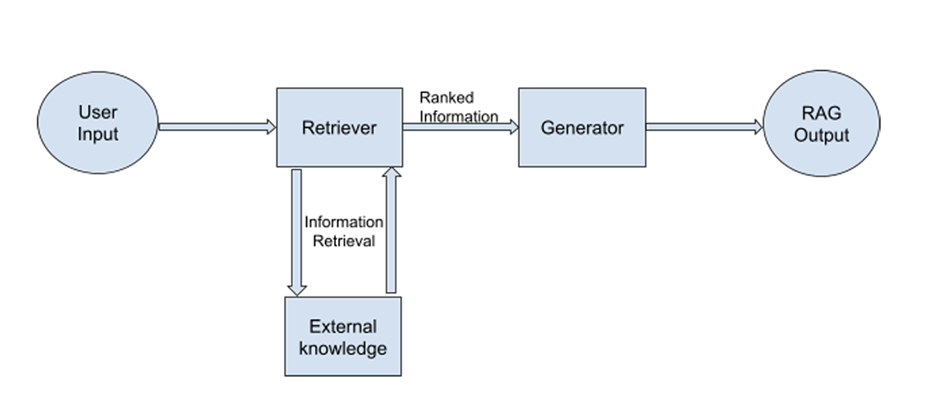
\includegraphics[width=0.8\linewidth]{Chapters/Figures/architeture_of_RAG_system.png} % Adjust width or use height
    \caption{ Basic architecture of a RAG system \cite{gupta2024comprehensivesurveyretrievalaugmentedgeneration}}
    \label{fig:architeture_of_RAG_system}
\end{figure}

RAG operates with two distinct types of memory parametric and non-parametric \cite{lewis2021retrievalaugmentedgenerationknowledgeintensivenlp}:
\begin{itemize}
    \item \textbf{Parametric memory}: Refers to the internal knowledge already present in the model's parameters during training, represented in the weight embeddings.

    \item \textbf{Non-parametric memory}: Refers to the external knowledge source that the model retrieves during inference. These external sources can include databases, web pages (e.g., Wikipedia), or structured knowledge graphs, enabling the model to answer queries with current or domain-specific information.
\end{itemize}
This distinction allows to combine static with dynamic information, significantly enhancing flexibility and accuracy.

RAG models can be classified as two main types, based on how they handle retrieved documents during the generation process \cite{20BNEURIPS2020_6b493230}:
\begin{itemize}
    \item \textbf{RAG-Sequence Model}: Only the retrieved document is used throughout the generation of an entire sentence or response.

    \item \textbf{RAG-Token Model}: This model allows retrieving different documents for each target token. It selects a distinct latent document for each generated token, retrieves the top \(k\) documents, and produces the output sequence probability for each document.
\end{itemize}

There are three main categories of RAG approaches \cite{21Bgao2024modularragtransformingrag}:
\begin{itemize}
    \item \textbf{Naïve RAG}: The first paradigm of RAG being adopted. It follows a process that includes indexing, retrieving, augmenting, and generating responses (see Figure ~\ref{fig:NaiveRAG}).

    \item \textbf{Advanced RAG}: In addition to the steps involved in Naïve RAG, pre-retrieval and post-retrieval processes are included to improve the quality of responses (see Figure ~\ref{fig:AdvancedRAG}).
    \begin{itemize}
        \item \textbf{Pre-retrieval process}: The main goal is to improve the quality of the content being indexed.
        \item \textbf{Post-retrieval process}: The main goal is to enhance the way the chunks retrieved are merged with the user query to form the prompt. Techniques such as re-ranking and prompt compression are used to achieve this. 
    \end{itemize}

    \item \textbf{Modular RAG}: Divides the retrieval and generation components into independent, interchangeable modules. This allows each module to be independently developed, optimized, or swapped out, enabling experimentation with various retrieval techniques and generation models.
\end{itemize}

\begin{figure}[htbp]
    \centering
    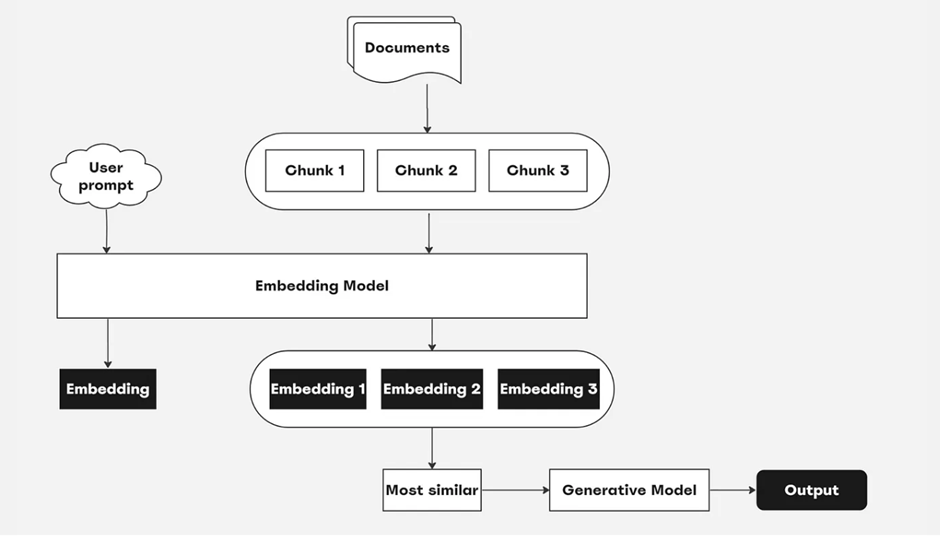
\includegraphics[width=0.8\linewidth]{Chapters/Figures/NaiveRAG.png} % Adjust width or use height
    \caption{ Naive RAG \cite{jayanth_blog}}
    \label{fig:NaiveRAG}
\end{figure}

\begin{figure}[htbp]
    \centering
    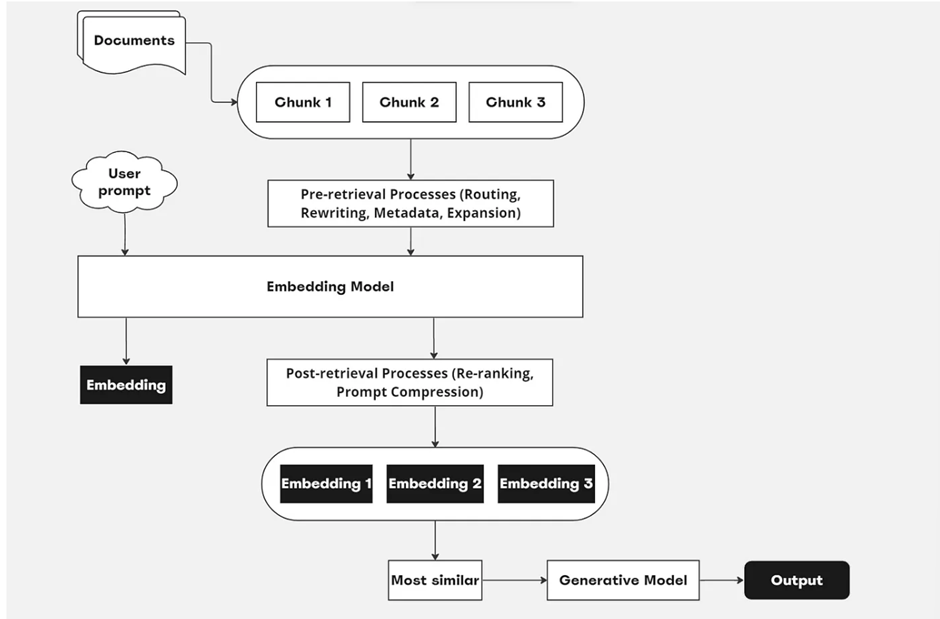
\includegraphics[width=0.8\linewidth]{Chapters/Figures/Advanced RAG.png} % Adjust width or use height
    \caption{ Advanced RAG \cite{jayanth_blog}}
    \label{fig:AdvancedRAG}
\end{figure}

\section{Systematic mapping studies}
\label{sec:systematic_mapping_studies}


Systematic mapping studies, also referred as scoping studies, are a structured and unbiased methodology for identifying, categorizing, and analyzing the existing literature on a specific research topic \cite{23BKeele2007}. The main goal is to give a wide overview of a research area, to understand the extent of existing studies and identify gaps in knowledge. This methodology consists of systematically searching the literature to determine which topics have been covered, where has been published and in what form \cite{22BPetersen2008}.
The systematic mapping studies are typically divided into three main stages: planning, conducting and discussion of results. Each stage has a defined process to ensure the reliability and validity of the study. We are going to implement a systematic mapping study to identify the current state of the art in the use of LLMs for requirements engineering, this way understanding better the gaps and possible improvements in the current state of the art.

\subsection{Planning stage}
The first part of the systematic mapping study is to define the research questions that will be driving the research. These questions are crucial, as they are going to guide the search process, help identify relevant studies and establish the focus of data extraction and analysis. Effective research questions, give an overview of the current practices regarding the specific topic and identifying current gaps in knowledge \cite{24BKitchenham2007}. 

Additionally, we must define the search strategy to guarantee a comprehensive coverage. This involves composing a search string with a set of keywords based on the main terms of the research questions and driven by their objectives. A properly designed search string assures a search process that is systematic, replicable and unbiased.

Inclusively, we define the inclusion and exclusion criteria with the focus on the research questions to ensure an appropriate and reliable classification. Inclusion criteria focus on determine studies that address the research questions while exclusion criteria filter out unrelated or irrelevant studies. For example:
 \begin{itemize}
    \item \textbf{Inclusion criteria:} Studies that respond to the main research question.
    \item \textbf{Exclusion criteria:} Studies that are in other languages then English.
 \end{itemize}

 \subsection{Conducting stage}
In this stage, implement the defined search strategy, by applying the search string in digital libraries and conducting the screening process. Articles that correspond to the exclusion criteria are excluded, similarly, those that provide relevant information, corresponding to the inclusion criteria, are included.

Studies can be considered unrelated to our research just by reading their title and abstract, therefore, they can be excluded without further reading. However, if the abstract isn’t clear if corresponds to research questions, the conclusions or any part of the full paper should be read to clarify how it should be classified. 

After the initial screening, data extraction is performed. Relevant information from the selected studies is collected, such as methodology implemented, conclusions, publication details, and relationship to the research questions.

Data extraction must be conducted systematically to guarantee the reliability and reproducibility of the results.

\subsection{Discussion of results}
Discussion phase involves analyzing the results of the conducting stage and the responses to the research questions, to gain a deeper understanding of state literature, identify the gaps, trends and underexplored areas on the topic. This phase includes three main tasks, analyzing trends, identifying gaps and documenting results. 

For example, a systematic study in natural language processing for requirements engineering might analyze the natural language processing tools being developed in the requirement engineering field, such as OICSI \cite{25BZhao2021}.

\section{Summary}
This chapter gives an overview of the main concepts to automating the creation of design models from requirements. It starts by introducing the importance of software modeling and the use of UML class diagrams to represent the structure of a system. 
Software modeling is explain with a focus on UML class diagrams, explaining their components, relationships, benefits for developers and stakeholders, and describing the design process, highlighting key steps such as requirement analysis, identifying relationships, defining multiplicity, adding attributes/methods, and refining the model.
The chapter then explores LLMs, describing their Transformer-based architecture and key components like multi head self-attention, embeddings and decoders.While LLMs have advanced NLP applications, they face challenges such as context limitations, hallucinations, and dependency on training data. To improve their performance in requirement modeling, two techniques are examined: prompt engineering (zero-shot, few-shot, and chain-of-thought prompting) and RAG, which integrates external knowledge to enhance accuracy.
Finally, the chapter discusses systematic mapping studies, a structured method for analyzing existing research. It describes the planning, conducting, and discussion stages of the study conducted in this work, which aims to identify gaps in LLM-based requirement modeling. These insights serve as the foundation for the research, helping define strategies to enhance LLM-driven software modeling automation.